\section{Scheduling}

A real-time scheduling system embodies the clock, the elements used in hardware processing and not to forget, the scheduler itself. Each task has their own schedulability in the system. This means that, depending on the characteristic of the scheduling algorithm, the tasks will first be accepted by the real-time system then fulfilled by the given or specified deadline of the task. This explains that a scheduling algorithm designates how tasks are being processed by the scheduling system. Each task will also be assigned its own description, deadline and an identifier which denotes their priorities. The selected scheduling algorithm determines how a particular task is assigned to its own priorities \cite{b9}.

\subsection{Static Versus Dynamic Scheduling}

Next, we come to the classification of real-time scheduling. A real-time scheduling can be sorted or divided into two parts. We can either have a static or a dynamic scheduling algorithm. Basically, their main difference is that a static scheduler (which also called pre-runtime scheduler) will dictate the priorities of the task before the system runs, meanwhile a dynamic scheduler (which also called on-line scheduler), will be determining the task priorities as the system runs by choosing one from the contemporaneous sets of ready tasks. The tasks are then accepted from the computing environment by the hardware parts in a real-time scheduling system and processed in real-time. The processing state is indicated by an output signal. A task deadline is the amount of time allotted to finish each assignment [9].
This indicates that a static scheduler constructs its decision for the scheduling literally at the time of compilation or technically at the point which a program is converted from source code to machine code. Thus, it requires a complete advance foreknowledge with respect to attributes of the task, for example, the maximum execution times, the precedence constraints, the mutual exclusion constraints, and not to forget the deadlines. On the other hand, for a dynamic scheduler, as the consequence for making its decision for scheduling at running time, this makes it adaptable to a changing task circumstance. This is due to their behaviour of only considering the current task requests. However, it is also worth noting that the amount of time and work required to find a schedule can be tremendous \cite{b3}. ``Fig.~\ref{fraction}'' is provided to have a clearer view between the distinctions stated.

\begin{figure}[htp]
    \centering
    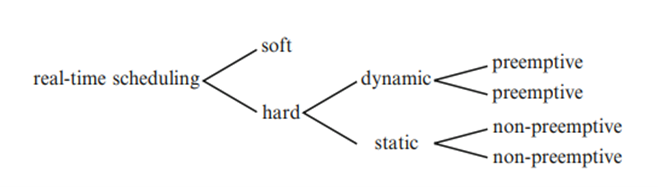
\includegraphics[width=7.5cm]{fraction}
    \caption{Fractions of real-time scheduling with comparison between dynamic and static scheduling \cite{b3}.}
    \label{fraction}
\end{figure}

Predominantly, the behaviour of the system is non-deterministic. As we can see on the figure shown before, the schedulers used in dynamic scheduler are preemptive while the schedulers used in static scheduler are non-preemptive. In non-preemptive scheduling, the task that is currently being executed will not gong to be interfered until it allows the allocation of the resources to be released or used. Hence, this makes non-preemptive scheduling very reasonable in a scenario where many short tasks are needed to be executed. Contradictorily, in preemptive scheduling, it is possible to have an interrupt during the process. As for example, the currently executing task could be preempted or interrupted if there exist a more urgent task which requests for a service \cite{b3}.

\subsection{Scheduling Problems}

Nowadays, most industrial control applications with real-time demands are made up of tasks from a variety types and constraints. These constraints require both types of processes, periodic and aperiodic. This may also differ for their criticality. The main objective of the kernel is to guarantee the schedulability of all critical tasks in worst-case conditions and give reasonable response times on the average for not only soft but also non-real-time tasks or process when dealing with hybrid task sets. 
As what is stated in the Murphy’s Law, "Anything that can go wrong will go wrong", meeting the requisite deadline will not always work possible to be achieved. On that account, extensive research of the scheduling algorithm is necessary to be organized for further verification. Dynamic scheduling algorithm can be implemented using two different techniques. It is either by assigning the deadline of the task based on their priority (earliest deadline) or assigning the completion time for each task by subtracting the processing time from the deadline (least laxity). As the consequence, we must understand the deadlines and the required task execution time in advance to ensure the processing elements execution times are being utilized efficiently \cite{b9}.

One of the major problems that we may encounter in the analysis of sporadic task systems is the concerns of unpredictability of the task requests. For periodic task systems, the set of task requests to be encountered is known a priori. However, there is by no means to determine which set of task requests would be encountered in irregular task systems. The key scheduling issue thus is on-line feasibility testing.  The system must decide if a new sporadic task can be accepted when it arrives at the node. Acceptance signifies that the job can be completed in the time between its arrival and its deadline without jeopardizing the deadlines of periodic tasks or previously accepted sporadic activities. The accepted task is then queued until it is selected to be processed by the local scheduler. Otherwise, another module of the scheduler in responsibility of dispatching this task to another computer in the distributed system can take refusal into account \cite{b5} and this is where we will study and observe the importance of server which closely related to the term of ‘Temporal Isolation’.
